% !TEX root = ../vr_st.tex

\subsection{Real projective spaces} \label{sub:first_critical_value_rpn}

\subsubsection{}

For any integer $n \geq 1$ and real number $r > 0$, let $\bS^n(r)$ be the \defn{$n$-sphere} of radius $r$ centered at the origin of $\R^{n+1}$.
We consider it equipped with the geodesic distance $d$.

The \defn{$n$-real projective space} $\rp^n(r)$ is the quotient space $\bS^n(r)$ by the antipodal map $x \mapsto -x$ for all $x \in \bS^n$.
We equip $\rp^n(r)$ with the quotient metric.
% \[
% d\big([x],[x']\big) =
% \min\set[\big]{d(x, x'), d(-x, x')}.
% \]

To simplify notation we denote $\bS(1)$ by $\bS^n$ and $\rp^n(2)$ by $\rp^n$.
Notice that $\diam(\bS^n) = \diam(\rp^n) = \pi$.

The inclusion of \(\mathbb{S}^n\) into \(\mathbb{S}^{n+1}\) as the equatorial $n$-sphere is equivariant with respect to the antipodal action.
Therefore, it induces an inclusion of \(\rp^n\) into \(\rp^{n+1}\).

%Since the \defn{infinite sphere} \(\mathbb{S}^\infty = \bigcup_n \mathbb{S}^n\) is contractible, its induced projection onto the \defn{real projective space} $\rp^\infty = \bigcup_n \rp^n$ defines its universal cover, so $\rp^\infty$ is a model for \(K(\Z/2, 1)\).

\subsubsection{}\label{sub:barcode_rpn}
% \anibal{This subsection is redundant if the subsection on barcode estimates is presented well. I placed it at the beginning of the section. Then the 3 examples will follow and use it to obtain the desired estimates.}

Consider the mod-\(2\) cohomology of \(\VR\rp^n\) and the linear cohomology operations defined by Steenrod squares \(\Sq^k_\ell \in \cO(\ell,\ell+k)\).
We respectively denote by $\alpha, \beta_\degp$ and $\gamma_{k + \ell}$ the first critical values of \(\VR\rp^n\), \(\rH_\degp(\VR\rp^n)\), and \(\img_{\Sq^k_\ell}\).

In \cref{subsub:rpn homotopy type}, \cref{subsub:beta_m_rpn} and \cref{subsub:gamma_rpn}, we will respectively prove that all three critical values are $\frac{2\pi}{3}$, when $1 \leq \degp \leq n$, $0 \leq k \leq \min\{\frac{n-1}{2}, \ell\} \leq n$ and $\binom{\ell}{k}$ is odd.

Applying results in \cref{subsub:barcode_general}, we obtain an estimate of the barcodes of $\rp^n$ and illustrate it in \cref{fig:sq barcodes}.
We illustrate it in \cref{fig:sq barcodes}, as this will be needed for estimating the bottleneck distance between barcodes.

\begin{figure}
	\centering
	\begin{tikzpicture}[scale=0.52]
	\begin{axis} [
		title = {\LARGE $\Hbarc{\degp}{\rp^n},\, \degp\leq n$},
		ticklabel style = {font=\Large},
		axis y line=middle,
		axis x line=middle,
		ytick={0.5,0.67,0.95},
		yticklabels={$\frac{\pi}{2}$,$\frac{2\pi}{3}$,$\pi$},
		xtick={0.5,0.67,0.95},
		xticklabels={$\frac{\pi}{2}$,$\frac{2\pi}{3}$,$\pi$},
		xmin=-0.015, xmax=1.1,
		ymin=0, ymax=1.1,]
		\addplot [mark=none] coordinates {(0,0) (1,1)};
		\addplot [thick,color=black!20!white,fill=black!30!white,
		fill opacity=0.4]coordinates {
			(0.67,0.95)
			(0.67,0.67)
			(0.95,0.95)
			(0.67,0.95)};
		\addplot [black!40!white,mark=none,dashed, thin] coordinates {(0,0.67) (0.67,0.67)};
		%\addplot [black!40!white,mark=none,dashed, thin] coordinates {(0,0.72) (0.72,0.72)};
		\addplot [black!40!white,mark=none,dashed, thin] coordinates {(0.67,0) (0.67,0.67)};
		\addplot[barccolor,mark=*] (0, 0.67) circle (2pt) node[above right,barccolor]{};%{\Large\textsf{1}};
		%\node[mark=none] at (axis cs:0.68,0.21){$\Hbarc{1}{\rp^n}$};
	\end{axis}
\end{tikzpicture}
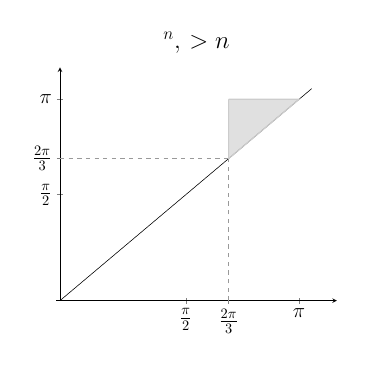
\begin{tikzpicture}[scale=0.52]
	\begin{axis} [
		title={\LARGE $\Hbarc{\degp}{\rp^n},\, \degp>n$},
		ticklabel style = {font=\Large},
		axis y line=middle,
		axis x line=middle,
		ytick={0.5,0.67,0.95},
		yticklabels={$\frac{\pi}{2}$,$\frac{2\pi}{3}$,$\pi$},
		xtick={0.5,0.67,0.95},
		xticklabels={$\frac{\pi}{2}$,$\frac{2\pi}{3}$,$\pi$},
		xmin=-0.015, xmax=1.1,
		ymin=0, ymax=1.1,]
		\addplot [mark=none] coordinates {(0,0) (1,1)};
		\addplot [thick,color=black!20!white,fill=black!30!white,
		fill opacity=0.4]coordinates {
			(0.67,0.95)
			(0.67,0.67)
			(0.95,0.95)
			(0.67,0.95)};
		\addplot [black!40!white,mark=none,dashed, thin] coordinates {(0,0.67) (0.67,0.67)};
		\addplot [black!40!white,mark=none,dashed, thin] coordinates {(0.67,0) (0.67,0.67)};
		% \addplot[barccolor,mark=*] (0, 0.67) circle (2pt) node[above right,barccolor]{\Large\textsf{1}};
		% \node[mark=none] at (axis cs:0.68,0.21){$\Hbarc{\degp}{\rp^n},\, \degp\geq 2$};
	\end{axis}
\end{tikzpicture}

\begin{tikzpicture}[scale=0.52]
	\begin{axis} [
		title = {\LARGE $\sqbarcl{k}{}{\rp^n},\, m \leq n$ and $\binom{m-k}{k}$ odd},
		ticklabel style = {font=\Large},
		axis y line=middle,
		axis x line=middle,
		ytick={0.5,0.67,0.95},
		yticklabels={$\frac{\pi}{2}$,$\frac{2\pi}{3}$,$\pi$},
		xtick={0.5,0.67,0.95},
		xticklabels={$\frac{\pi}{2}$,$\frac{2\pi}{3}$,$\pi$},
		xmin=-0.015, xmax=1.1,
		ymin=0, ymax=1.1,]
		\addplot [mark=none] coordinates {(0,0) (1,1)};
		\addplot [thick,color=black!20!white,fill=black!30!white,
		fill opacity=0.4]coordinates {
			(0.67,0.95)
			(0.67,0.67)
			(0.95,0.95)
			(0.67,0.95)};
		\addplot [black!40!white,mark=none,dashed, thin] coordinates {(0,0.67) (0.67,0.67)};
		%\addplot [black!40!white,mark=none,dashed, thin] coordinates {(0,0.72) (0.72,0.72)};
		\addplot [black!40!white,mark=none,dashed, thin] coordinates {(0.67,0) (0.67,0.67)};
		\addplot[barccolor,mark=*] (0, 0.67) circle (2pt) node[above right,barccolor]{};
        %{\Large$\geq$\textsf{1}};
	\end{axis}
\end{tikzpicture}
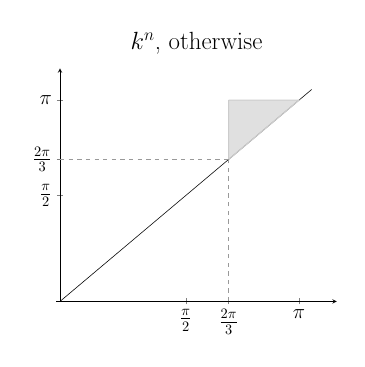
\begin{tikzpicture}[scale=0.52]
	\begin{axis} [
		title={\LARGE $\sqbarcl{k}{}{\rp^n}$, otherwise},
		ticklabel style = {font=\Large},
		axis y line=middle,
		axis x line=middle,
		ytick={0.5,0.67,0.95},
		yticklabels={$\frac{\pi}{2}$,$\frac{2\pi}{3}$,$\pi$},
		xtick={0.5,0.67,0.95},
		xticklabels={$\frac{\pi}{2}$,$\frac{2\pi}{3}$,$\pi$},
		xmin=-0.015, xmax=1.1,
		ymin=0, ymax=1.1,]
		\addplot [mark=none] coordinates {(0,0) (1,1)};
		\addplot [thick,color=black!20!white,fill=black!30!white,
		fill opacity=0.4]coordinates {
			(0.67,0.95)
			(0.67,0.67)
			(0.95,0.95)
			(0.67,0.95)};
		\addplot [black!40!white,mark=none,dashed, thin] coordinates {(0,0.67) (0.67,0.67)};
		\addplot [black!40!white,mark=none,dashed, thin] coordinates {(0.67,0) (0.67,0.67)};
	\end{axis}
\end{tikzpicture}
	\caption{\emph{Top row:} the $\degp^\th$ persistent homology barcode of $\rp^n$.
		When $1\leq \degp \leq n$, the barcode consists of one $(0,\frac{2\pi}{3})$ and potentially some bars dominated by $(\frac{2\pi}{3}, \pi)$.
		\emph{Bottom row:} the degree-$(k+\ell)$ component of the $\Sq^k$-barcode of $\rp^n$.
		The leftmost barcode contains at least one $(0,\frac{2\pi}{3})$ and potentially some bars dominated by $(\frac{2\pi}{3}, \pi)$.
		See \cref{sub:barcode_rpn}.
	}
	\label{fig:sq barcodes}
\end{figure}

\subsubsection{}
\label{subsub:rpn homotopy type}

In certain intervals, the homotopy type of the Vietoris--Rips complex of the $n$-sphere and $n$-projective space is known.
This information is presented in \cite[Thm.~4.5]{adams2022metric}:
%\label{prop:RPn}{\rm \cite[Thm.~4.5]{adams2022metric}.}
For $r \in (0,\frac{2\pi}{3} ]$,
\[
\VR_r\rp^n \simeq \rp^n,
\]
and the homotopy type of $\VR_r\rp^n$ changes after $\tfrac{2\pi}{3}$.
In other words,

\medskip\proposition
The first critical value of \(\VR\rp^n\) is \(\alpha = \frac{2\pi}{3}\).

\subsubsection{}
\label{subsub:beta_m_rpn}

We apply \cref{sub:general_barcodes} to prove the following proposition.

\medskip\proposition
The first critical value of the $\degp^{\th}$ homology of $\VR\rp^n$ is $\beta_m=\frac{2\pi}{3}$ for any $1\leq m\leq n$.

\begin{proof}%[Proof of \cref{subsub:beta_m_rpn}.]
	It follows from \cite{katz1983filling} that the filling radius of $\rp^n$ is $\frac{\pi}{3}$ for any $n \geq 1$.
	By \cref{subsub:foundamental_bar_rpn_lemma}, $\beta_m\leq \tfrac{2\pi}{3}$.
    On the other hand, $\beta_\degp\geq \alpha = \tfrac{2\pi}{3}$.
    This finishes the proof.
	% Additionally, we have that
	% \[
	% \rp^1 \subset \rp^2 \subset \dots \subset \rp^n,
	% \]
	% with $\rp^\degp$ generating the $\degp^\th$ mod 2 homology of $\rp^n$ for every $1 \leq \degp \leq n$.
	% This implies that $\beta_{\degp, n} \leq \beta_{\degp, n'}$ for any $n\leq n'$ and $\degp$.
	% Applying \cref{subsub:foundamental_bar_rpn_lemma}, we obtain that $\beta_{m,n} = \delta_1 = \tfrac{2\pi}{3},$ for any $n\geq 1$ and $1 \leq m \leq n$.
\end{proof}

\subsubsection{}
\label{subsub:gamma_rpn}

Denoting by \(\gamma_{\ell+k}\) the first critical value of \(\img_{\Sq^k_\ell}\) on \(\VR\rp^n\), we have the following.

\medskip\proposition
If $0 \leq k \leq \min\{\frac{n-1}{2}, \ell\} \leq n$ and $\binom{\ell}{k}$ is odd, then $\gamma_{k+\ell} = \tfrac{2\pi}{3}$.

\begin{proof}
	Since the Vietoris--Rips complex $\VR_r\rp^n$ retains the homotopy type of $\rp^n$ for $r \in [0,\tfrac{2\pi}{3})$, $\Sq^k(\sigma^\ell) = \binom{\ell}{k}\sigma^{\ell+k}$ generates a bar in the $\Sq^k_\ell$--barcode that is born at $0$ and stay alive until the non-trivial degree-$(\ell+k)$ class $\sigma^{k+\ell}$ dies at $\tfrac{2\pi}{3}$.
	Thus, the first critical value of $\gamma_{k+\ell} \leq \tfrac{2\pi}{3}$.
	On the other hand, $\gamma_{k+\ell} \geq \alpha = \tfrac{2\pi}{3}$ the first critical value of $\VR\rp^n$.
	Thus, $\gamma_{k+\ell} = \tfrac{2\pi}{3}$.
	\anibal{We do not know that it dies. \ling{I modified the definition of $\gamma_\bullet$, so it does die now.}}
\end{proof}
